\documentclass[]{article}
\usepackage{lmodern}
\usepackage{amssymb,amsmath}
\usepackage{ifxetex,ifluatex}
\usepackage{fixltx2e} % provides \textsubscript
\ifnum 0\ifxetex 1\fi\ifluatex 1\fi=0 % if pdftex
  \usepackage[T1]{fontenc}
  \usepackage[utf8]{inputenc}
\else % if luatex or xelatex
  \ifxetex
    \usepackage{mathspec}
  \else
    \usepackage{fontspec}
  \fi
  \defaultfontfeatures{Ligatures=TeX,Scale=MatchLowercase}
\fi
% use upquote if available, for straight quotes in verbatim environments
\IfFileExists{upquote.sty}{\usepackage{upquote}}{}
% use microtype if available
\IfFileExists{microtype.sty}{%
\usepackage[]{microtype}
\UseMicrotypeSet[protrusion]{basicmath} % disable protrusion for tt fonts
}{}
\PassOptionsToPackage{hyphens}{url} % url is loaded by hyperref
\usepackage[unicode=true]{hyperref}
\hypersetup{
            pdfborder={0 0 0},
            breaklinks=true}
\urlstyle{same}  % don't use monospace font for urls
\usepackage{graphicx,grffile}
\makeatletter
\def\maxwidth{\ifdim\Gin@nat@width>\linewidth\linewidth\else\Gin@nat@width\fi}
\def\maxheight{\ifdim\Gin@nat@height>\textheight\textheight\else\Gin@nat@height\fi}
\makeatother
% Scale images if necessary, so that they will not overflow the page
% margins by default, and it is still possible to overwrite the defaults
% using explicit options in \includegraphics[width, height, ...]{}
\setkeys{Gin}{width=\maxwidth,height=\maxheight,keepaspectratio}
\IfFileExists{parskip.sty}{%
\usepackage{parskip}
}{% else
\setlength{\parindent}{0pt}
\setlength{\parskip}{6pt plus 2pt minus 1pt}
}
\setlength{\emergencystretch}{3em}  % prevent overfull lines
\providecommand{\tightlist}{%
  \setlength{\itemsep}{0pt}\setlength{\parskip}{0pt}}
\setcounter{secnumdepth}{0}
% Redefines (sub)paragraphs to behave more like sections
\ifx\paragraph\undefined\else
\let\oldparagraph\paragraph
\renewcommand{\paragraph}[1]{\oldparagraph{#1}\mbox{}}
\fi
\ifx\subparagraph\undefined\else
\let\oldsubparagraph\subparagraph
\renewcommand{\subparagraph}[1]{\oldsubparagraph{#1}\mbox{}}
\fi

% set default figure placement to htbp
\makeatletter
\def\fps@figure{htbp}
\makeatother


\date{}

\begin{document}

\subsection{Hard-Sphere Molecular
Dynamics}\label{hard-sphere-molecular-dynamics}

In this section we introduce the concepts and methods needed to perform
molecular dynamics simulations of hard spheres. While these techniques
are not generally useful, in that they do not apply to the ``soft''
potentials that are of greater practical interest, they serve a purpose
for us now. Hard-sphere dynamics is the dynamics of billiards, or
marbles, so their behavior is very familiar to us. While it is not a
trivial matter to implement an efficient HS MD algorithm, once it is in
place very little ``tuning'' is needed to make hard-sphere MD
simulations work robustly---correctly programmed HS MD simulations are
very forgiving of the user. And in implementing a HS MD simulation one
encounters and must come to understand almost all of the basic elements
that make up any molecular simulation. Hard-sphere molecular dynamics
simulations provide us with a basis for presentation and discussion of
these simulation elements.

Once we have introduced the HS MD algorithm, we will move on to basic
simulation elements, including boundary conditions, averaging and error
estimation, the structure of a simulation, and initialization.

\paragraph{Hard-sphere dynamics}\label{hard-sphere-dynamics}

Hard spheres undergo impulsive, pairwise collisions. Never do three or
more spheres collide simultaneously, all meeting at exactly the same
time, so the collision dynamics can always be handled one pair at a
time. When hard spheres collide they experience an infinite force over
an infinitesimal time, yielding an impulse (product of force and time)
that is finite. This impulse imparts an equal and opposite change in
momentum to the two colliders. As shown in Fig.~\ref{fig:force}, the force is
directed along the centers of the two atoms, and of course acts to push
them away from each other. The magnitude of the impulse is governed by
conservation of energy. If we write the momentum change of each atom in
terms of the impulse , such that
\begin{align*}
  &{\bf{p}}_1^{\rm new} = {\bf{p}}_1^{\rm old} + \Delta {\bf{p}}\\
  &{\bf{p}}_2^{\rm new} = {\bf{p}}_2^{\rm old} - \Delta {\bf{p}}
\end{align*}
The only energy involved is that due to the kinetic energies of the
spheres. Conservation of energy requires
\[\frac{1}{{{m_1}}}{\left| {{\bf{p}}_1^{\rm new}} \right|^2} + \frac{1}{{{m_2}}}{\left| {{\bf{p}}_2^{\rm new}} \right|^2} = \frac{1}{{{m_1}}}{\left| {{\bf{p}}_1^{\rm old}} \right|^2} + \frac{1}{{{m_2}}}{\left| {{\bf{p}}_2^{\rm old}} \right|^2}\]
The equation is sufficient to specify the magnitude of $\Delta {\bf{p}}$. Taking its
direction as described in Fig.~\ref{fig:force}, we have
\[\Delta {\bf{p}} = \frac{{2{m_1}{m_2}}}{{{m_1} + {m_2}}}\frac{{{{\bf{v}}_{12}} \cdot {{\bf{r}}_{12}}}}{{{\sigma ^2}}}{{\bf{r}}_{12}}\]
To illustrate the plausibility of this expression, consider two limiting
cases. In a glancing collision, where the two spheres barely touch, the
dot product ${\bf v}_{12}\cdot{\bf r}_{12}$ approaches zero and very little impulse is applied to
either. In the opposite case, where they particles suffer a head on
collision, the impulse is (taking the masses equal, and noting $|{\bf r}_{12}|=\sigma$ at
collision) $\Delta {\bf{p}} = {{\bf{p}}_2} - {{\bf{p}}_1}$, and the spheres swap velocities (each reversing velocity,
for example, if they approach with the same speed as each other).

\begin{figure}
  \centering
  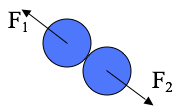
\includegraphics[width=\textwidth]{HSMD_figures/image001}
  \caption{\label{fig:force}Forces at collision.}
\end{figure}
  

\paragraph{Hard-sphere kinematics}\label{hard-sphere-kinematics}

When the spheres are not colliding they move in free flight; no forces
act on them and they do not accelerate. Thus over a collision-free
interval of time the position advances according to
\[{\bf{r}}(t + \Delta t) = {\bf{r}}(t) + {\bf{v}}(t)\Delta t\]
For such simple motion it is possible to solve analytically for the time
of collision between two given spheres. The time interval $Delta t$ to the next
collision satisfies
\[{\left| {{{\bf{r}}_2}(t + \Delta t) - {{\bf{r}}_1}(t + \Delta t)} \right|^2} = {\sigma ^2}\]
That is, the square distance between the spheres at the collision time
is equal to the collision diameter $\sigma$. Expansion of this formula leads to
a quadratic equation in $\Delta t$
\[|{{\bf{v}}_{12}}{|^2}{(\Delta t)^2} + 2({{\bf{v}}_{12}} \cdot {{\bf{r}}_{12}})(\Delta t) + (|{{\bf{r}}_{12}}{|^2} - {\sigma ^2}) = 0\]
As shown in Fig.~\ref{fig:approaches}, one of three situations can arise:

\begin{itemize}
\item If $({\bf v}_{12}\cdot {\bf r}_{12})$ is positive, the spheres are moving apart and will never collide. 
\item If $({\bf v}_{12}\cdot {\bf r}_{12})$ is negative, the spheres are approaching, but will not necessary collide
(indicated by a negative discriminant of the quadratic equation).
\item Finally, they may be approaching and on a collision course ($({\bf v}_{12}\cdot {\bf r}_{12})$ is negative
and the discriminant is positive).
\end{itemize}

\begin{figure}
  \centering
  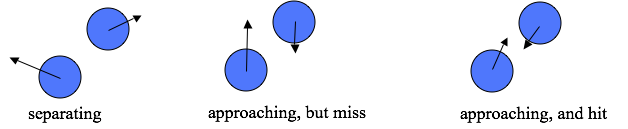
\includegraphics[width=\textwidth]{HSMD_figures/image030}
  \caption{\label{fig:approaches}Collision-approach cases.}
\end{figure}


\paragraph{Integration strategy}\label{integration-strategy}

The time evolution of a system of hard spheres can be traced by handling
each collision in sequence. The process is a simple repetition of
finding the next colliding pair, advancing all spheres to the time of
collision of this pair, handling the collision dynamics of the pair, and
moving on to detect the next collision. Conceptually, and in practice,
it is worthwhile to have in mind some finite interval of time, δt; the
aim is to advance to the system from the initial time through this time
interval, handling all intervening collisions in sequence. Completion of
the interval signals an appropriate point for examination of the system
and accumulation simulation averages (one could take this assessment at
each collision, but such a scheme unnecessarily restricts the sampling
of configurations to those in which one pair is colliding). The process
is depicted schematically in Fig.~\ref{fig:integration}.

\begin{figure}
  \centering
  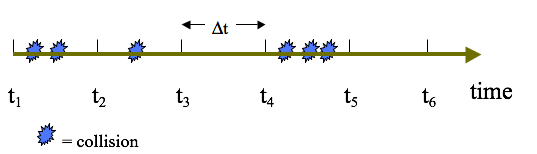
\includegraphics[width=\textwidth]{HSMD_figures/image037}
  \caption{\label{fig:integration}Constant-timestep integration through collisions.}
\end{figure}

The process of stepping through collisions to cross a fixed interval of
time can be implementing using a recursive strategy. One has a method
(or subroutine)---call it doStep---that takes as its argument an
interval of time. The method is constructed so that it advances the
system across the specified interval, handling the intervening
collisions, so that when it returns the system is at the end of the
given time interval. The recursive strategy is as follows: doStep
detects the next collision, advances the system to that time and handles
the dynamics, and then calls itself with the remainder of the time
interval as an argument. The termination condition for the recursion
occurs when doStep does not detect a collision occurring in the time
interval passed to it.

% Illustration 5 is an applet that demonstrates the collision-detection
% process. It is a simple simulation of two-dimensions hard-disks. At each
% point in the simulation, the next pair to collide is indicated with red
% and blue coloring. Note that not every collision is shown explicitly, as
% the image is re-drawn only at the end of each time interval $\delta t$.


Significant efficiency can be realized in the algorithm through intelligent
maintenance of a collision list. For this purpose it is helpful to have
in mind some fixed ordering of the atoms in a list. The ordering is
completely arbitrary, and need not change ever during the simulation
(although one might wish to do otherwise, as discussed in another
chapter). Each atom links to the next one up and the next one down the
list; Fig.~\ref{fig:ordering} describes the concept for a six-atom list. The
ordering of atoms in this manner is useful not only for hard-particle
simulations of the type we examine here, but also in more conventional
molecular dynamics and Monte Carlo simulations. Now, with the atoms
ordered in this fashion, we track collisions by having each atom
maintain a record of the next atom it is scheduled to collide,
considering only those atoms up-list from it. If atom 3 is on a
collision course with atom 1, it is the job of atom 1, not atom 3, to
keep hold of that fact. Each atom also records the amount of time that
until it meets its collision partner. For example, consider the scenario
presented in Fig.~\ref{fig:collisionTracking}. Atom 1 expect to collide with atom 3 in 1.2
fs; atom 2 expects to collide with atom 4 in 0.7 fs; atom 3 with atom 5
in 0.1 fs; and so on. No atom is uplist of atom 6, so it anticipates no
collision. A simple traversal of the collision list indicates that atom
3 has the smallest collision interval, so 3 and 5 collide next. These
are highlighted in red and blue, just as done in the applet of
Illustration 5. Note that atom 5 sees only its impending collision with
atom 6; the 3-5 collision comes about from the information held by atom
3.

\begin{figure}
  \centering
  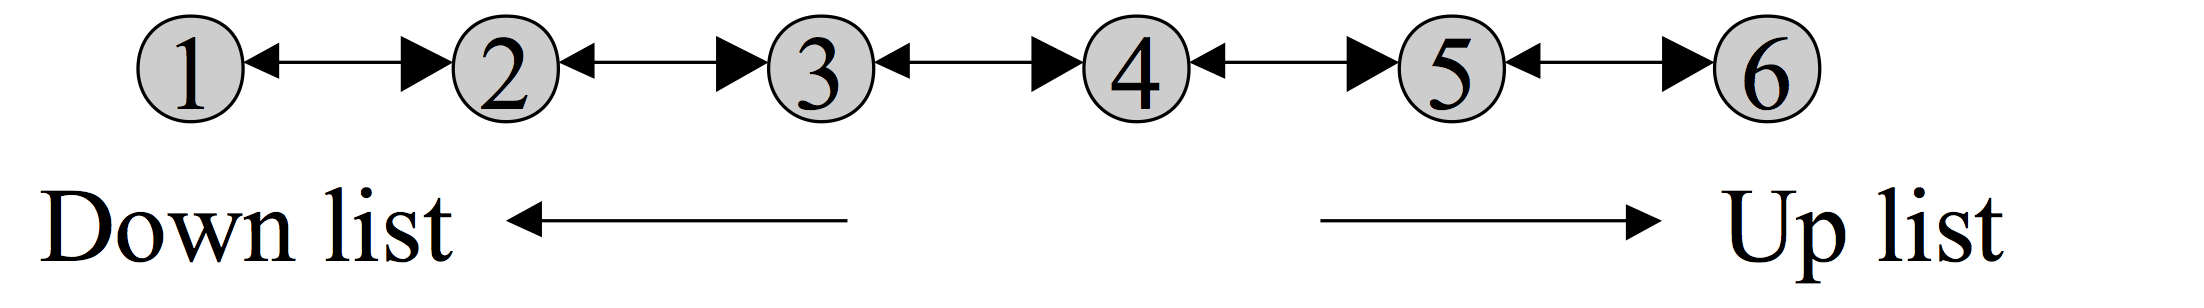
\includegraphics[width=\textwidth]{HSMD_figures/image040}
  \caption{\label{fig:ordering}Ordering of atoms for tracking collisions.}
\end{figure}


With this list in place it is a very simple matter to detect the next
collision. The problem then is to ensure that it is properly updated
with each collision, using minimal effort. First, after advancing the
system 0.1 fs to the 3-5 collision and dealing with their collision
dynamics, all collision times must be decremented by the amount of time
advanced. The 2-4 collision time, for example, is reduced to 0.6 fs.
Note first that most collision pairs do not have to be re-assessed in
light of the 3-5 collision. The trajectories of 2 and 4 are unchanged,
so only the only update for that pair is the decrement of their
collision. However, there are some subtleties that must be handled
correctly. Upon collision, it is (of course) necessary to update the
collision partners of 3 and 5, finding the minimum time of collision of
each with each atom uplist of them. It is also necessary to look at all
atoms downlist of 3 and 5 that were previously on a collision course
with either. For example, in Illustration 7 atom 1 was scheduled to
collide with 3 in 1.2 fs. Since atom 3 is now on a different course,
atom 1 must be checked against \emph{all} of its uplist atoms for its
next collision. It is also necessary to check all downlist atoms for new
collisions with atoms 3 and 5, as their changed trajectory may now lead
the to collide with, for example, atom 2 before 2 hits atom 4. A
possible scenario is diagrammed in Illustration 8

\begin{figure}
  \centering
  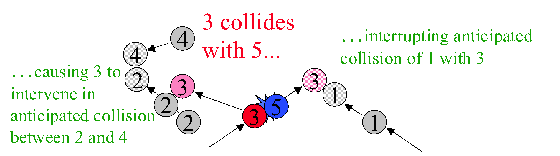
\includegraphics[width=\textwidth]{HSMD_figures/image042}
  \caption{\label{fig:collisionTracking}Tracking of collision partners.}
\end{figure}

From this description, maintenance of the collision list seems like a
complex process. It is not all that bad, and could be much worse.
Additional efficiencies can be brought into this process at the cost of
additional complexity, but we will postpone this detailed discussion to
another time. The simple alternative of checking all pairs at every
collision is much too inefficient to serve as a viable algorithm. The
efficiencies gained in the basic collision detection algorithm discussed
here certainly justify the bit of effort needed to sort through all the
scenarios needed to maintain the list.

\end{document}
